\documentclass[10pt]{beamer}

\usepackage{setup}
\usepackage[vlined]{algorithm2e}
\SetAlFnt{\scriptsize}

\title{Time Warp Simulation on Multi-core Processors and Clusters}
\author{
    Douglas A. Weber \\
    Masters Thesis Defense \\
    Advisor: Professor Philip A. Wilsey
}
\institute{University of Cincinnati}
\date{March XX, 2016}

\begin{document}

\begin{frame}
  \titlepage
\end{frame}

\begin{frame}{Discrete Event Simulation}
    \begin{itemize}
        \item Three main components
            \begin{itemize}
                \item State variables
                \item Simulation clock
                \item Pending event set
            \end{itemize}
        \bigskip
        \item Unprocessed events stored in pending event set
        \item Events processed in time stamp order
        \item Simulation clock and state variables updated only when event occurs
    \end{itemize}
\end{frame}

\begin{frame}{Parallel Discrete Event Simulation}

    \begin{columns}[c]

    \begin{column}{0.5\textwidth}
        \begin{itemize}
            \item Model system as a set of Logical Processes (LPs)
            \item Events exchanged between LPs
        \end{itemize}
    \end{column}

    \begin{column}{0.5\textwidth}
        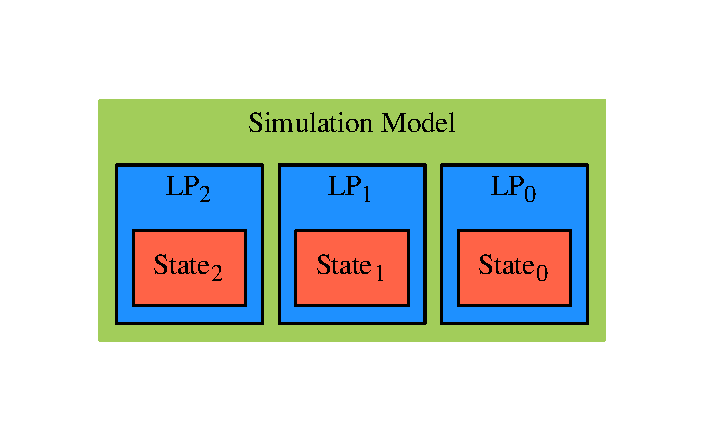
\includegraphics[width=\textwidth]{../figs/graphviz/pdes.pdf}
    \end{column}

    \end{columns}

    \begin{block}{Possible Causality Violations}

        \begin{columns}[T]

        \begin{column}{0.4\textwidth}
            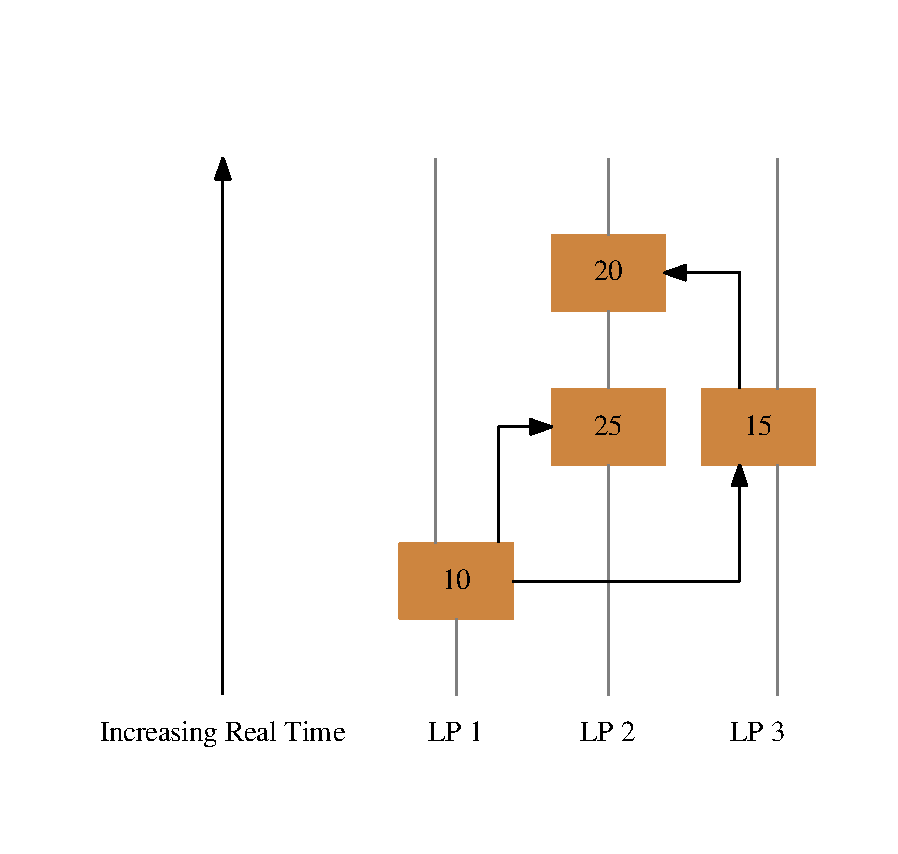
\includegraphics[width=\textwidth]{../figs/graphviz/causality.pdf}
        \end{column}

        \begin{column}{0.6\textwidth}
            \begin{itemize}
                \item Events can be received \emph{and} processed out of order
                \item Two solutions
                    \begin{itemize}
                        \item Conservative and Optimistic
                    \end{itemize}
            \end{itemize}
        \end{column}

        \end{columns}

    \end{block}

\end{frame}

\begin{frame}{Time Warp}
    \begin{block}{Optimistic Mechanism}
        \bigskip
        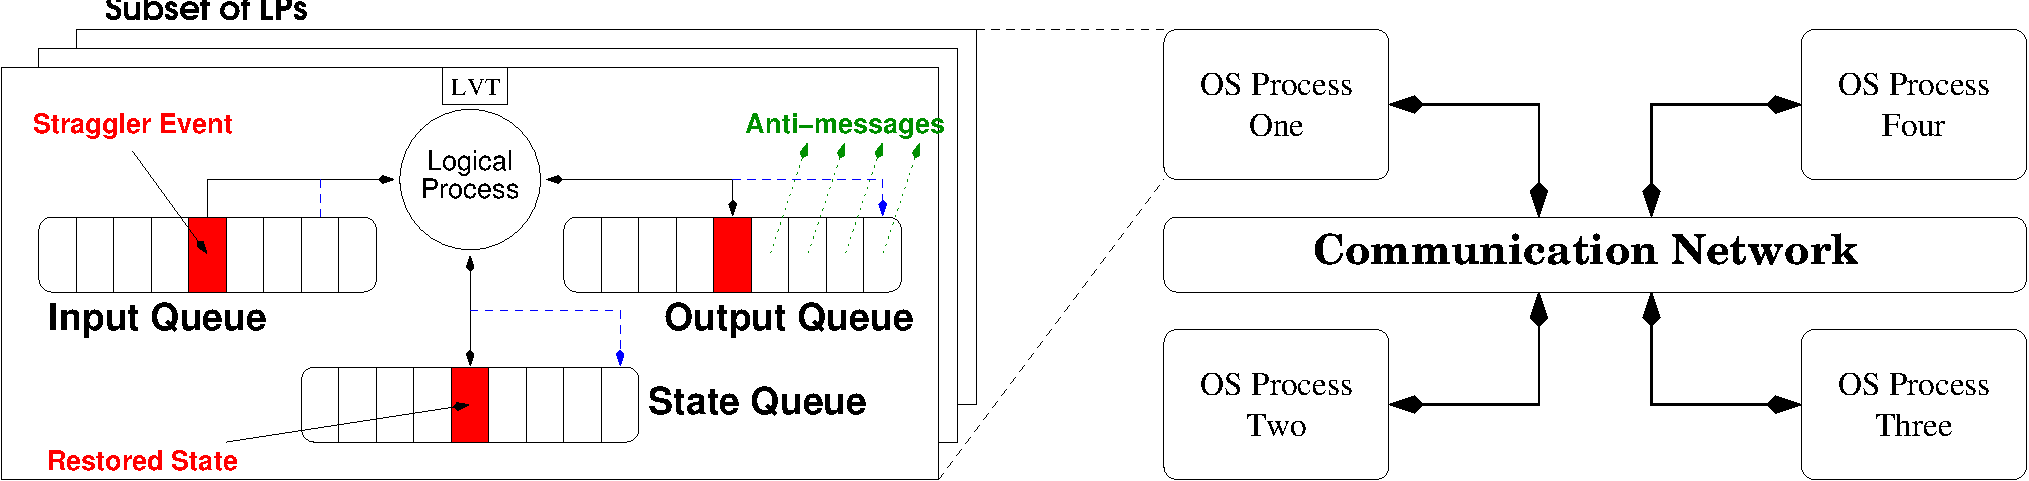
\includegraphics[width=\textwidth]{../figs/timeWarp.pdf}
        \bigskip
        \begin{itemize}
            \item Rollback Mechanism
                \begin{itemize}
                    \item State Restoration, Anti-Messages
                \end{itemize}
            \item Local Virtual Time (LVT) \& Global Virtual Time (GVT)
            \item Fossil Collection
        \end{itemize}
    \end{block}
\end{frame}

\begin{frame}{\textsc{warped2} Process}
        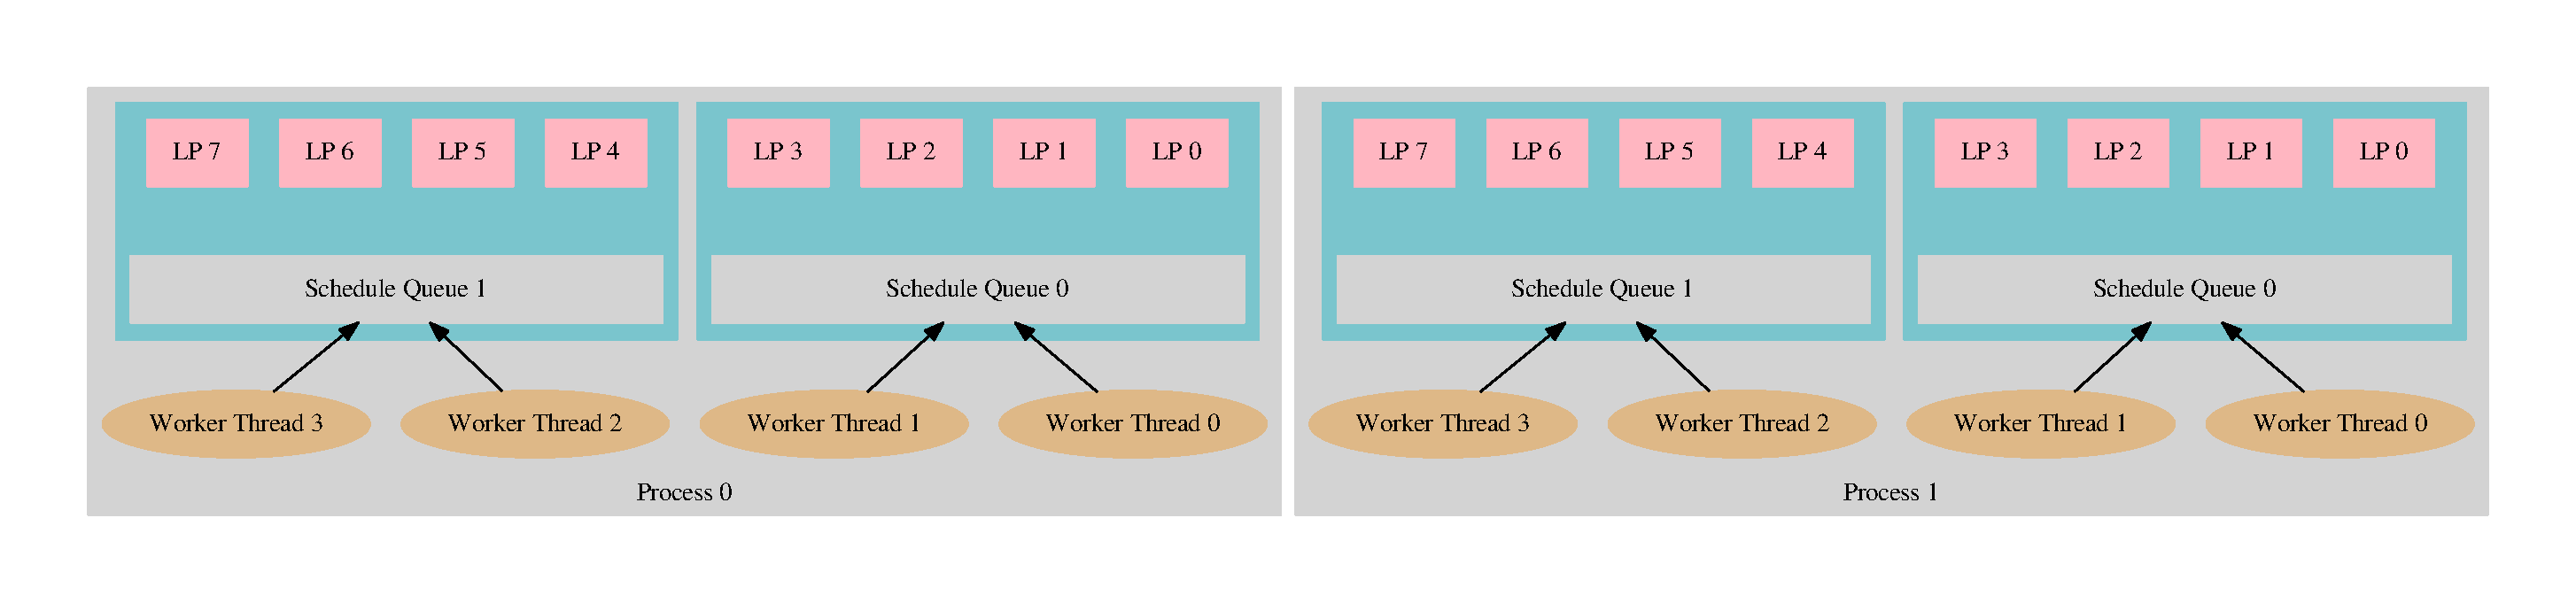
\includegraphics[width=\textwidth]{../figs/graphviz/partitioning.pdf}
        \begin{itemize}
            \item Worker Threads and Manager Thread
            \item LTSF Queues/Worker Thread - Contention vs Rollbacks
            \item LP Partitioning
        \end{itemize}
\end{frame}

\begin{frame}{Event Scheduling and Processing}
    \begin{columns}

        \begin{column}{0.4\textwidth}

            \begin{block}{Worker Threads}
            \bigskip
            
            \begin{algorithm}[H]
                \DontPrintSemicolon
                \SetKw{Continue}{continue}
                \SetKwFunction{getNextEvent}{getNextEvent}

                \While{termination not detected}{
                    $e \gets \getNextEvent{}$\;
                    $lp \gets$ receiver of $e$\;\;

                    \If{$e <$ last processed event for $lp$}{
                        rollback $lp$\;
                    }
                    \;
                    \If{$e$ is an anti-message}{
                        cancel event with $e$\;
                        schedule new event for $lp$\;
                        \Continue\;
                    }
                    \;
                    process event $e$\;
                    save state of $lp$\;
                    send new events\;
                    \;
                    move $e$ to processed queue\;
                    replace scheduled event for $lp$\;
                }
            \end{algorithm}

            \end{block}

        \end{column}

        \begin{column}{0.6\textwidth}
            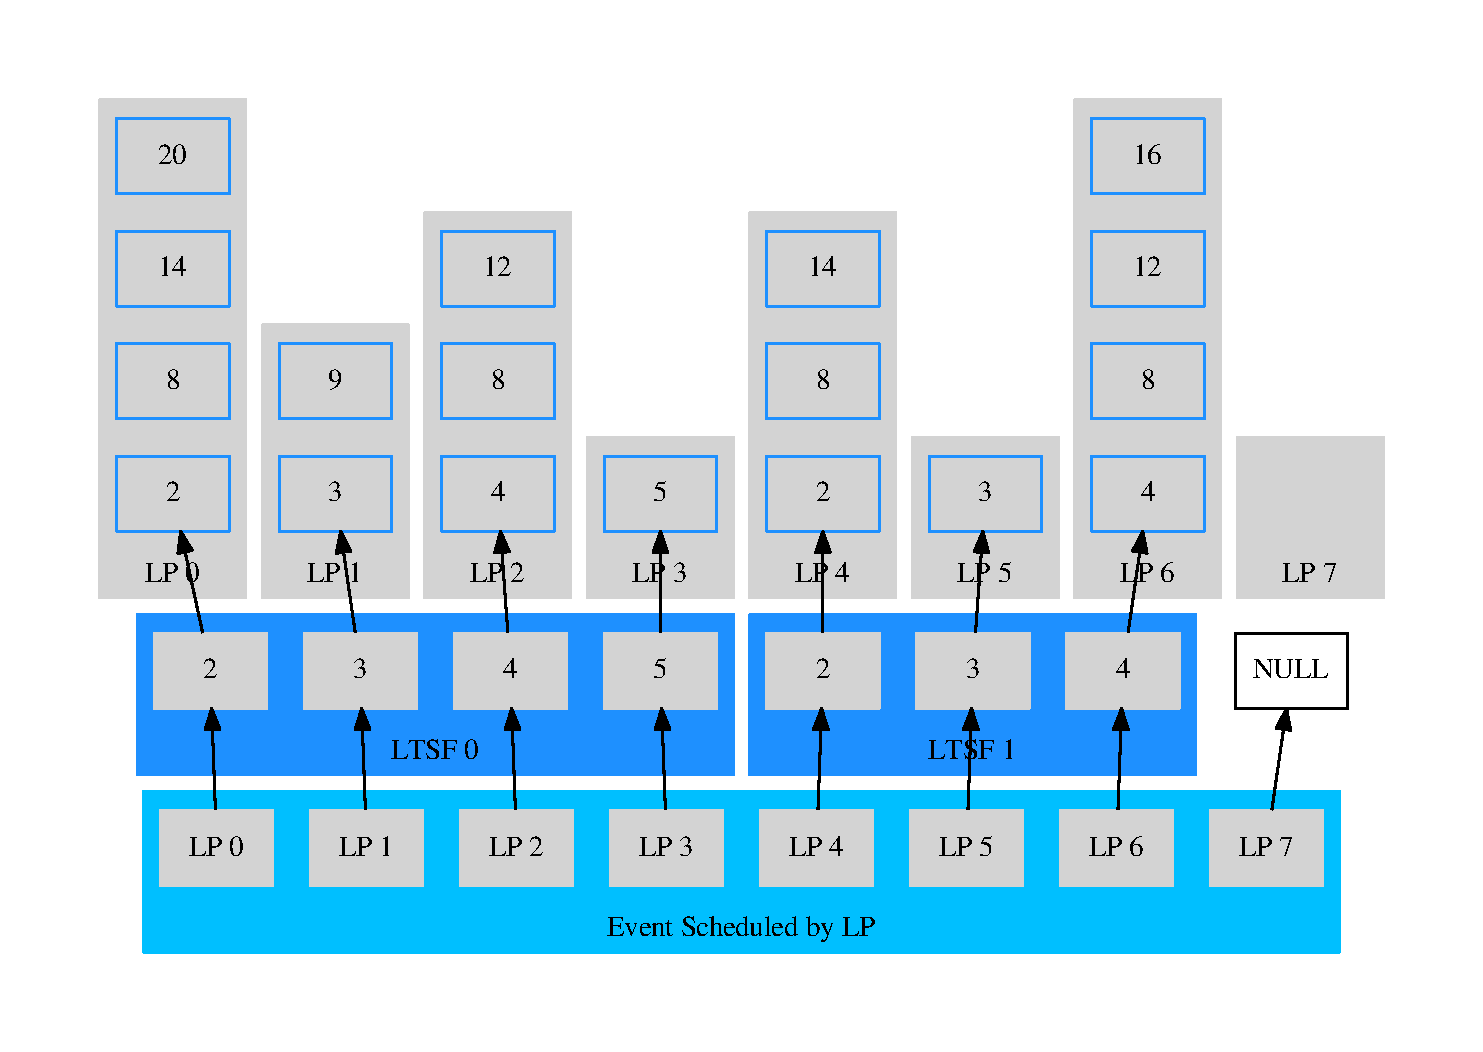
\includegraphics[width=\textwidth]{../figs/graphviz/pending_event_set.pdf}
            \begin{itemize}
                \item Unprocessed and Processed Queues
                \item Scheduling to LTSF
                \item Rollbacks
            \end{itemize}
        \end{column}

    \end{columns}
\end{frame}

\begin{frame}{Sharing LTSF Queues}
    \begin{minipage}{0.5\textwidth}
        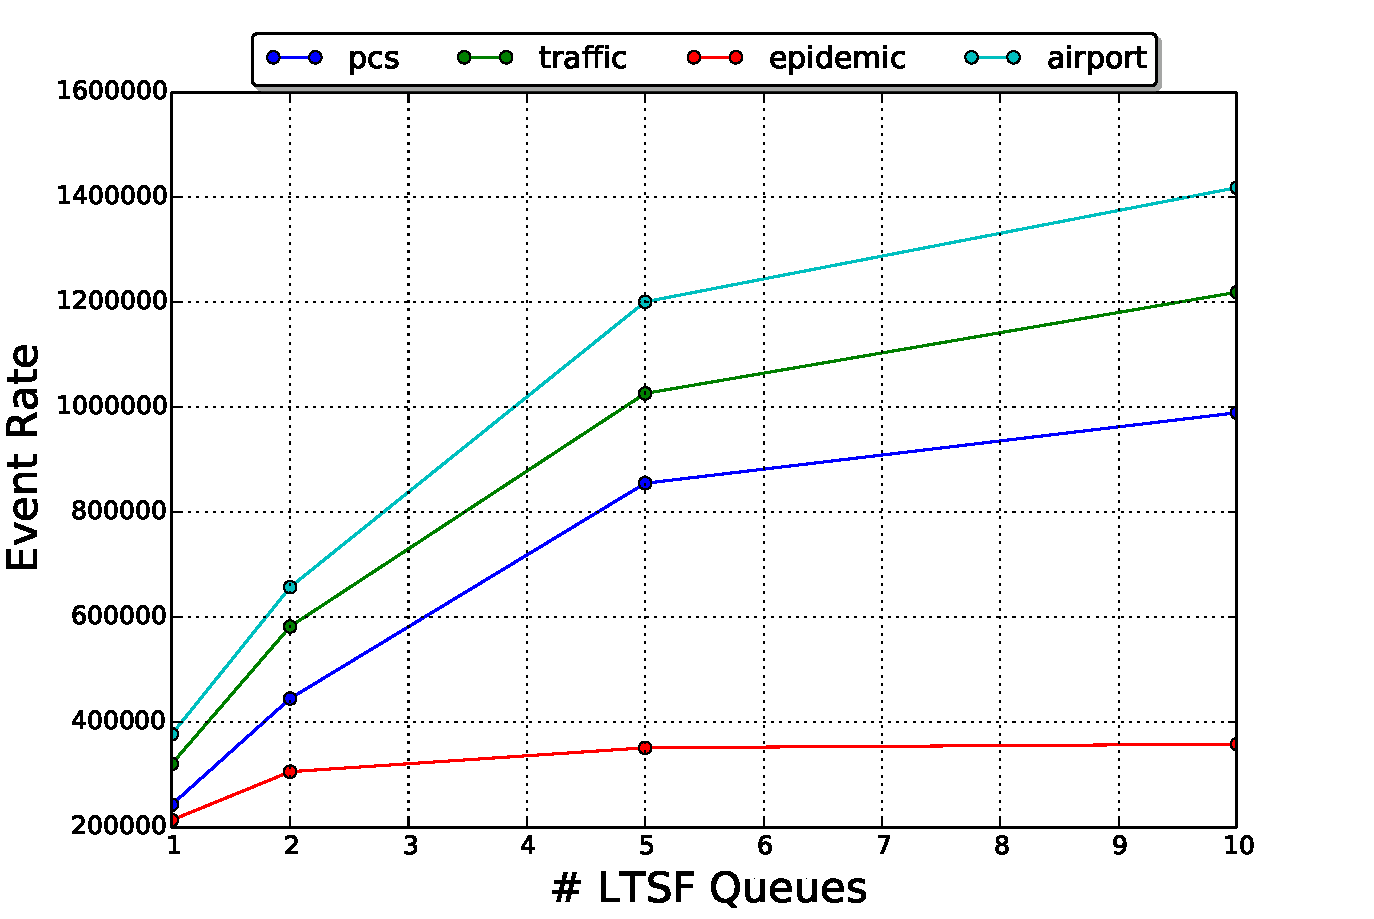
\includegraphics[width=\textwidth]{../figs/pending_event_set/ltsf_event_rate.pdf}
        $$EventRate={CommitedEvents \over Runtime}$$
    \end{minipage}%
    \begin{minipage}{0.5\textwidth}
        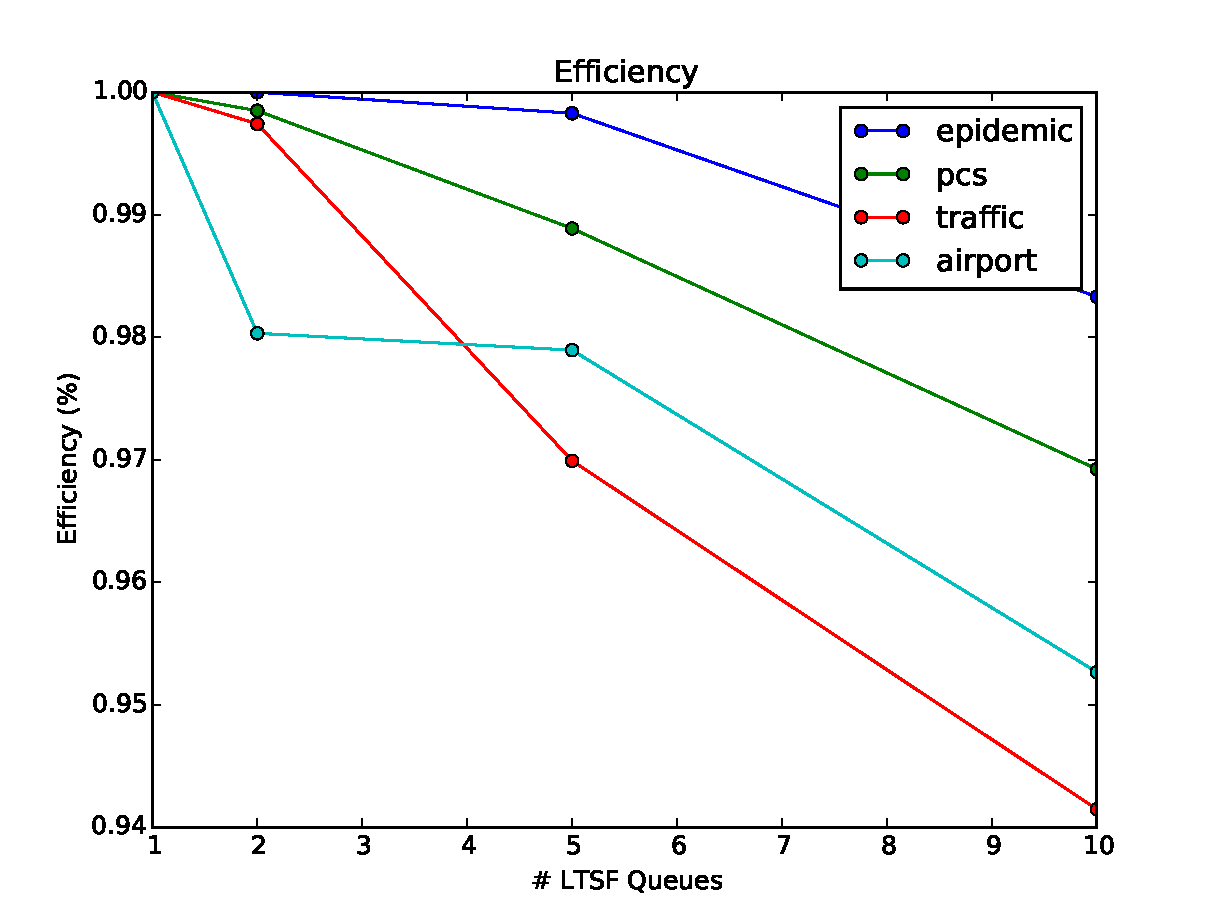
\includegraphics[width=\textwidth]{../figs/pending_event_set/ltsf_efficiency.pdf}
        $$Efficiency={CommittedEvents \over ProcessedEvents}*100 \%$$
    \end{minipage}
    \begin{block}{Reducing contention more important than reducing rollbacks}\end{block}
\end{frame}

\begin{frame}{Periodic State Saving - Overview}
    \begin{block}{Save state only once every $N$ events}
        \bigskip
        \centering
        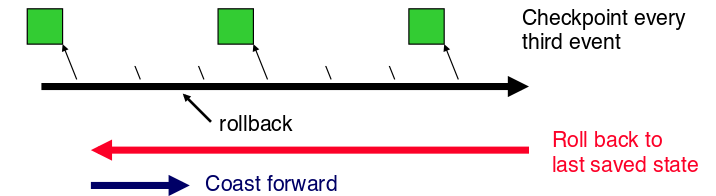
\includegraphics[width=0.6\textwidth]{../figs/pss.png}
        \bigskip
        \begin{itemize}
            \item Not all states available to roll back to
            \item Must "Coast Forward" to reproduce state
            \item Increases time to rollback
            \item Decrease time to save states and reduce memory footprint
        \end{itemize}
    \end{block}
\end{frame}

\begin{frame}{Periodic State Saving - SMP Machine}
    \begin{block}{Intel\textsuperscript{\textregistered} Xeon\textsuperscript{\textregistered} X5675}
        \smallskip
        \begin{minipage}{0.5\textwidth}
            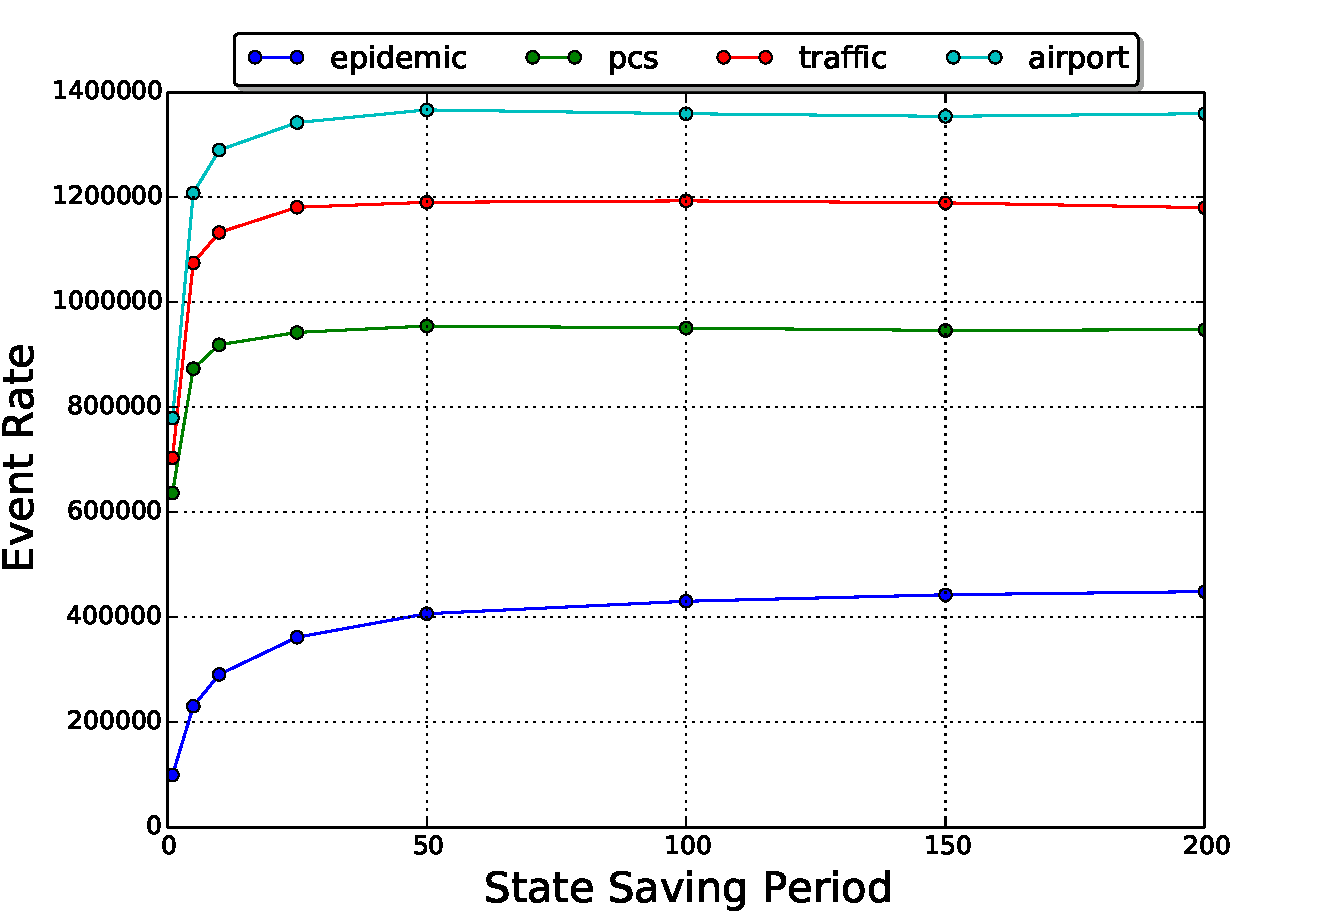
\includegraphics[width=\textwidth]{../figs/state_saving/bc/eventrate.pdf}
        \end{minipage}%
        \begin{minipage}{0.5\textwidth}
            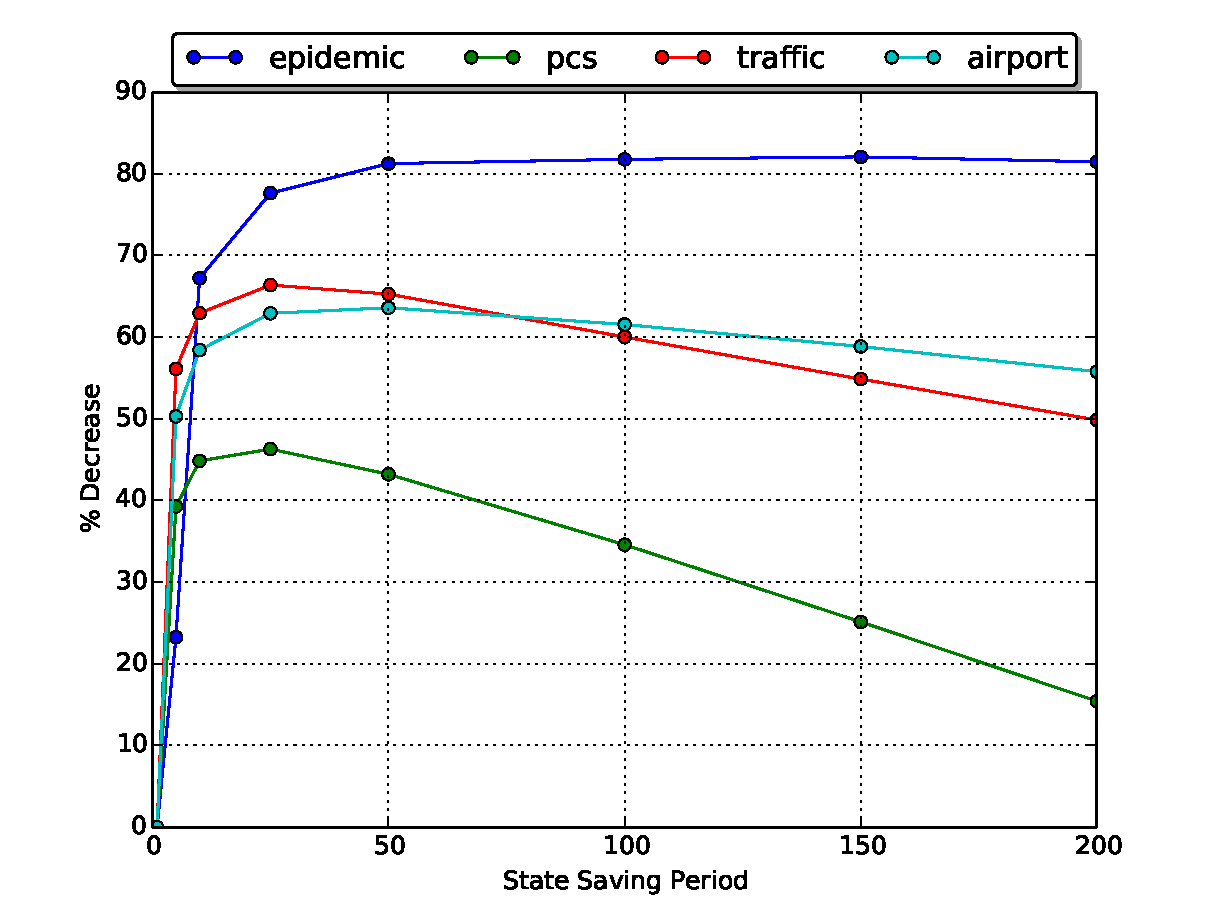
\includegraphics[width=\textwidth]{../figs/state_saving/bc/percent_memory_decrease.pdf}
        \end{minipage}
    \end{block}
\end{frame}

\begin{frame}{Periodic State Saving - Cluster}
    \begin{block}{8 Nodes - Intel\textsuperscript{\textregistered} Xeon\textsuperscript{\textregistered} E5410}
        \smallskip
        \begin{minipage}{0.5\textwidth}
            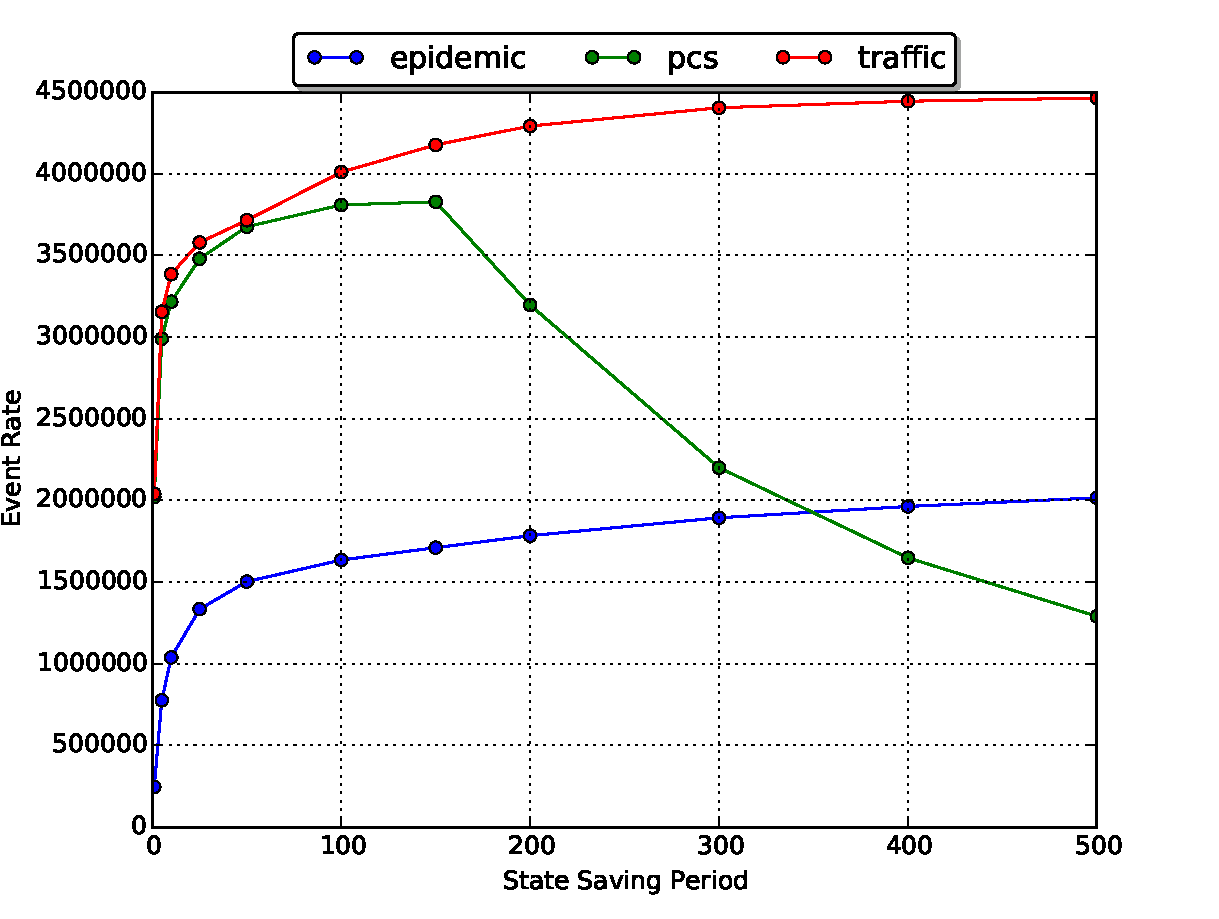
\includegraphics[width=\textwidth]{../figs/state_saving/beowulf/eventrate_500.pdf}
        \end{minipage}%
        \begin{minipage}{0.5\textwidth}
            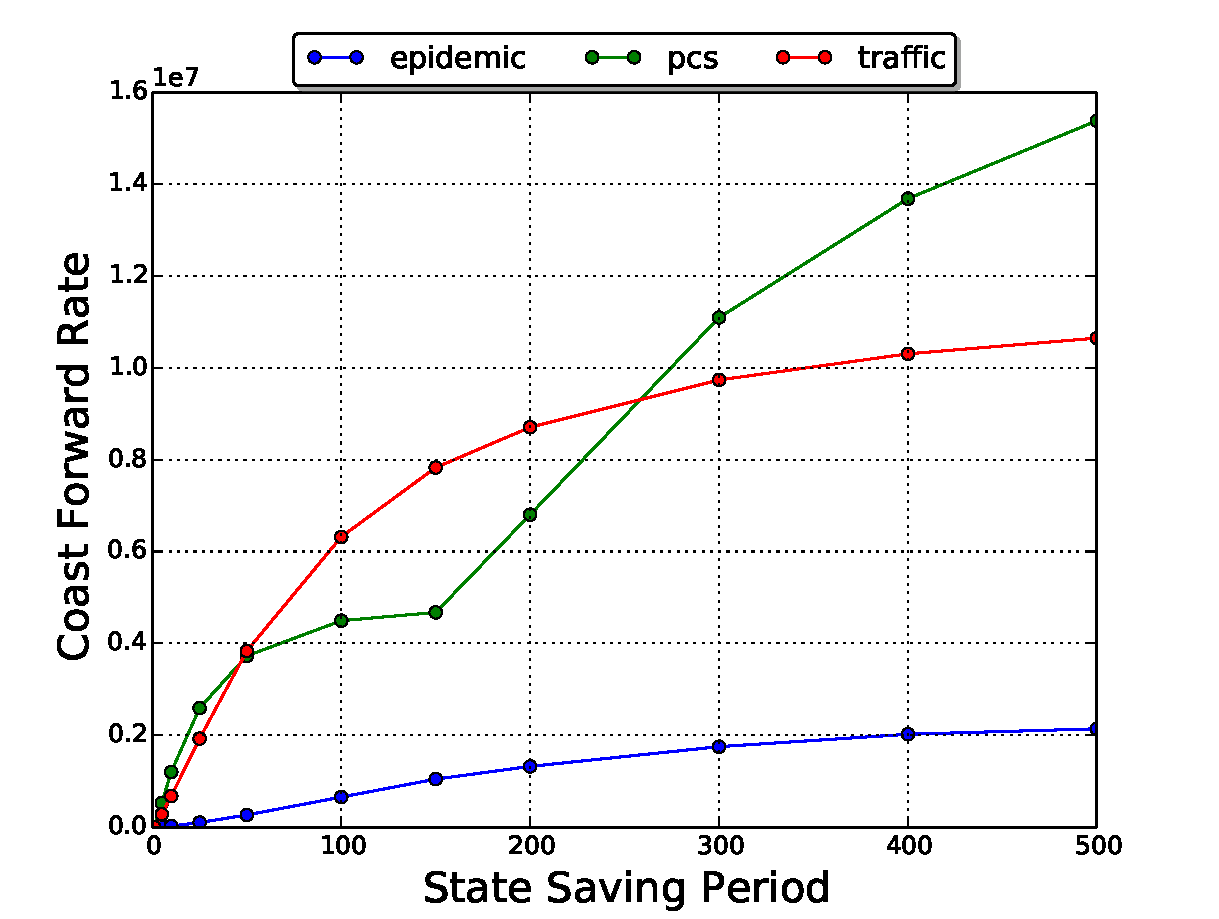
\includegraphics[width=\textwidth]{../figs/state_saving/beowulf/cf_rate_500.pdf}
        \end{minipage}
    $$ CoastForwardRate = {CoastForwardEvents \over Rollbacks} * RollbackRate $$
    \end{block}
\end{frame}

\begin{frame}{Communication Model}
    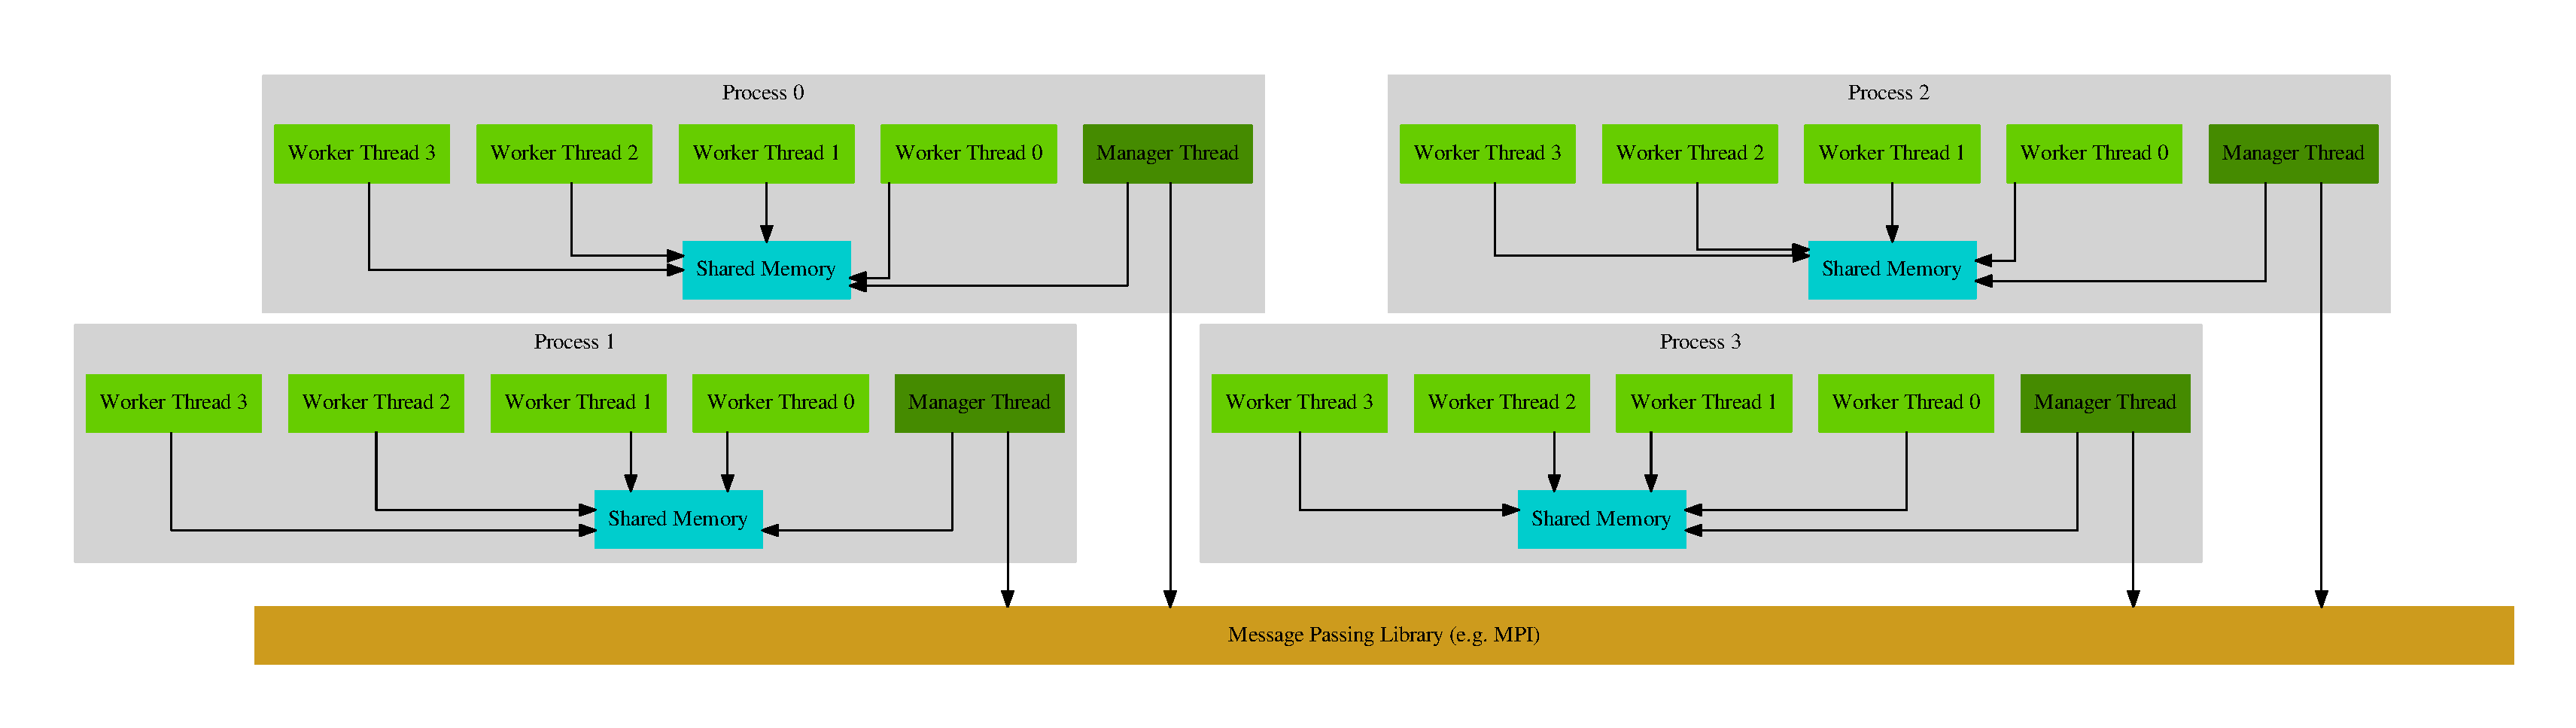
\includegraphics[width=\textwidth]{../figs/graphviz/warped_communication.pdf} \\
    Thread Message Passing Models
    \begin{itemize}
        \item Single threaded
        \item Funnelled
        \item Serialized
        \item Multiple
    \end{itemize}
\end{frame}

\begin{frame}{Communication Model - Traffic Model}
    \begin{minipage}{0.5\textwidth}
        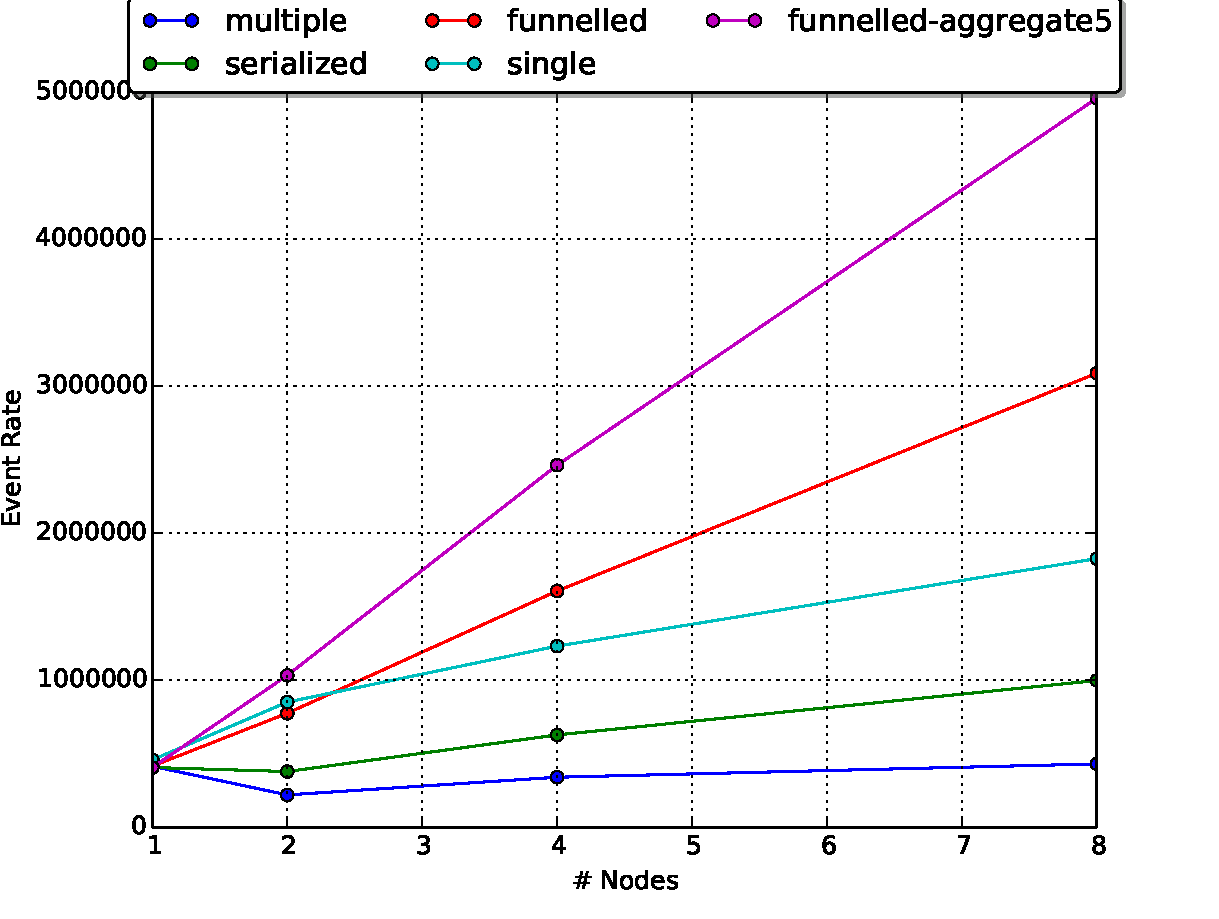
\includegraphics[width=\textwidth]{../figs/partitioning_communication/communication_traffic_eventrate.pdf}
    \end{minipage}%
    \begin{minipage}{0.5\textwidth}
        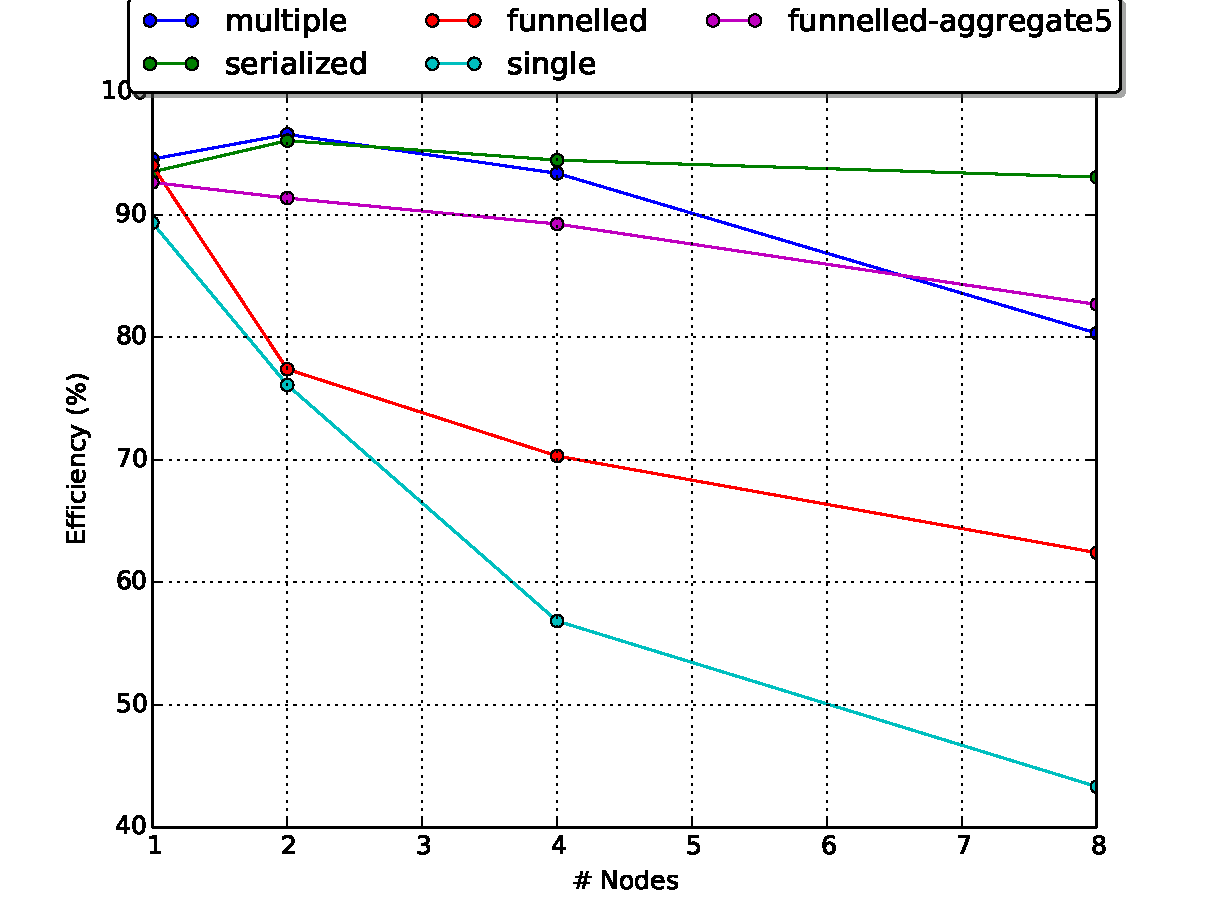
\includegraphics[width=\textwidth]{../figs/partitioning_communication/communication_traffic_efficiency.pdf}
    \end{minipage}
    \begin{itemize}
        \item Funneled/Single - Minimal Synchronization, High Latency
        \item Serialized/Multiple - Lots of Synchronization , Low Latency
        \item Performance will vary with model and partitioning.
    \end{itemize}
\end{frame}

\begin{frame}{Message Aggregation}
    \begin{itemize}
        \item Wait for $N$ messages with same destination \emph{process} and send together
        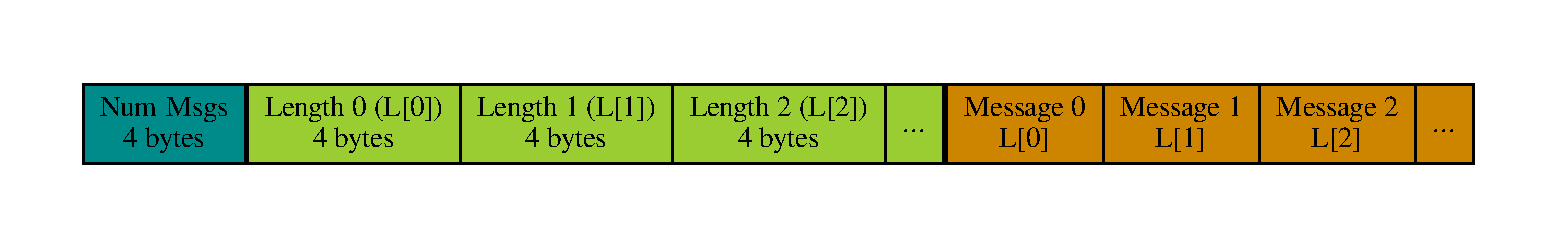
\includegraphics[width=\textwidth]{../figs/graphviz/aggregation_format.pdf}
        \item Pros
            \begin{itemize}
                \item Single buffer allocated for multiple messages
                \item Latency shared by multiple messages
                \item Events destined for same LP may be sent together
            \end{itemize}
        \item Cons
            \begin{itemize}
                \item May increase event latency too high
            \end{itemize}
    \end{itemize}
\end{frame}

\begin{frame}{Message Aggregation - Traffic Model}
    \begin{minipage}{0.5\textwidth}
        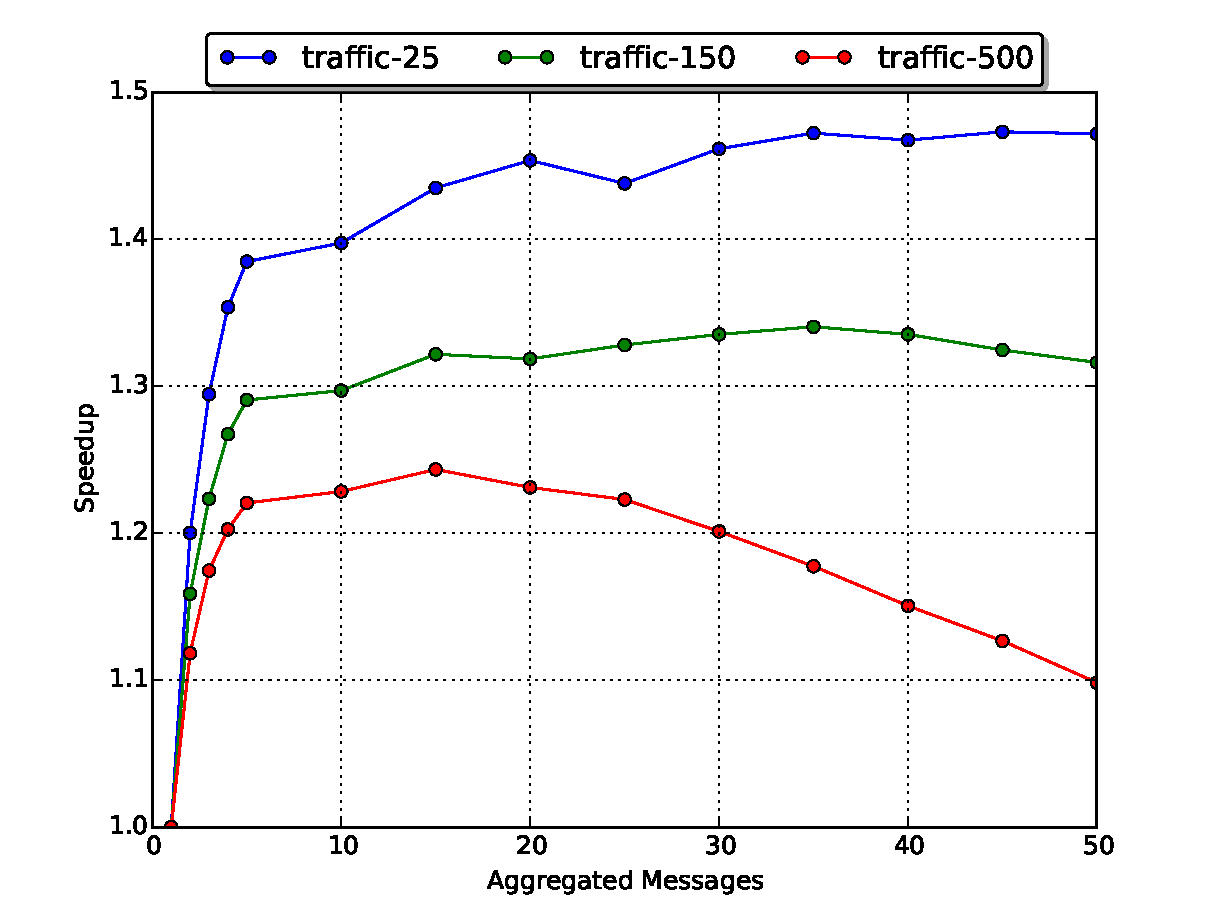
\includegraphics[width=\textwidth]{../figs/partitioning_communication/aggregate_traffic_speedup.pdf}
    \end{minipage}%
    \begin{minipage}{0.5\textwidth}
        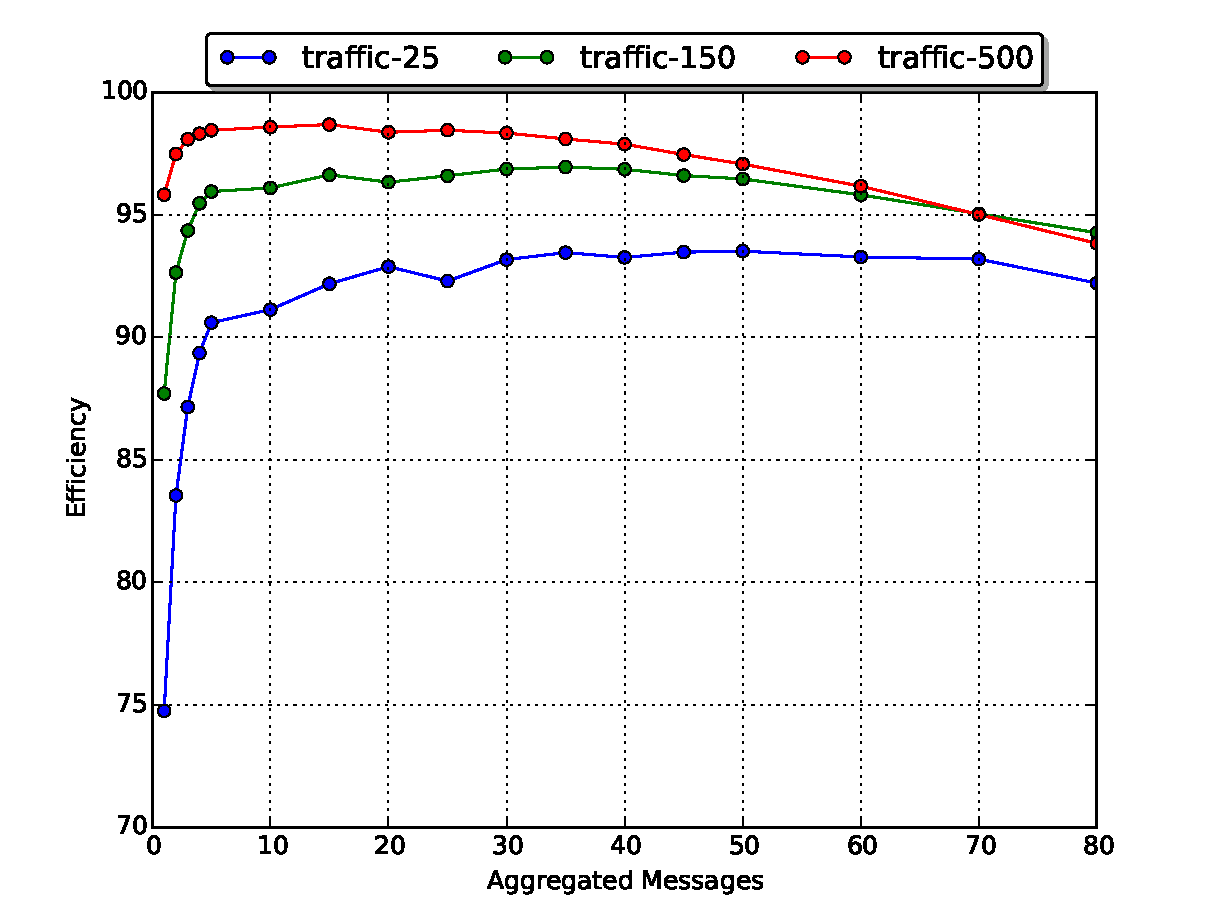
\includegraphics[width=\textwidth]{../figs/partitioning_communication/aggregate_traffic_efficiency.pdf}
    \end{minipage}
    \begin{itemize}
        \item Best with small number of aggregated events
        \item Different behavior with different state saving periods
    \end{itemize}
\end{frame}

\begin{frame}{Message Aggregation - More Observations}

    \begin{columns}

    \begin{column}{0.5\textwidth}
        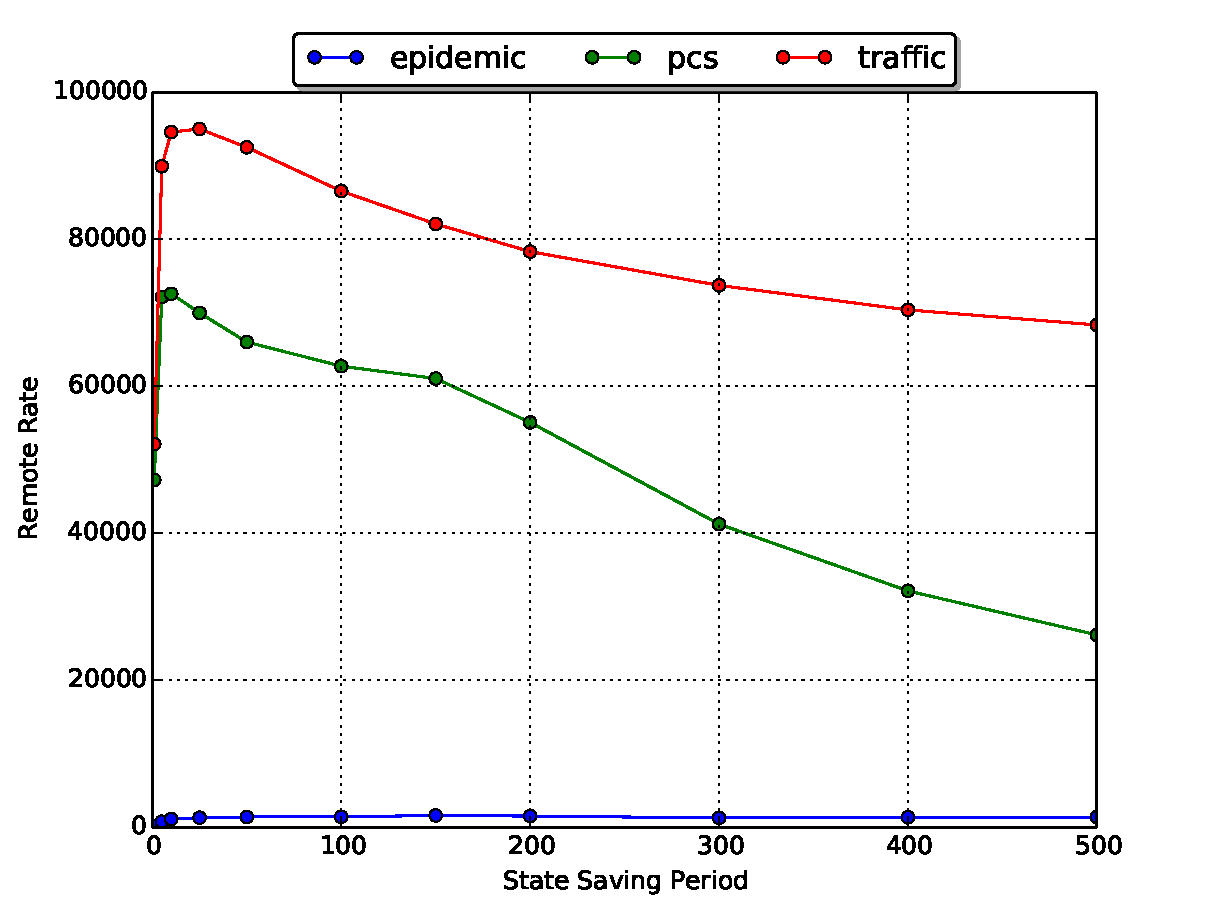
\includegraphics[width=\textwidth]{../figs/state_saving/beowulf/remote_rate.pdf}
        \begin{itemize}
            \item Faster rate of remote events better
        \end{itemize}
    \end{column}

    \begin{column}{0.5\textwidth}
        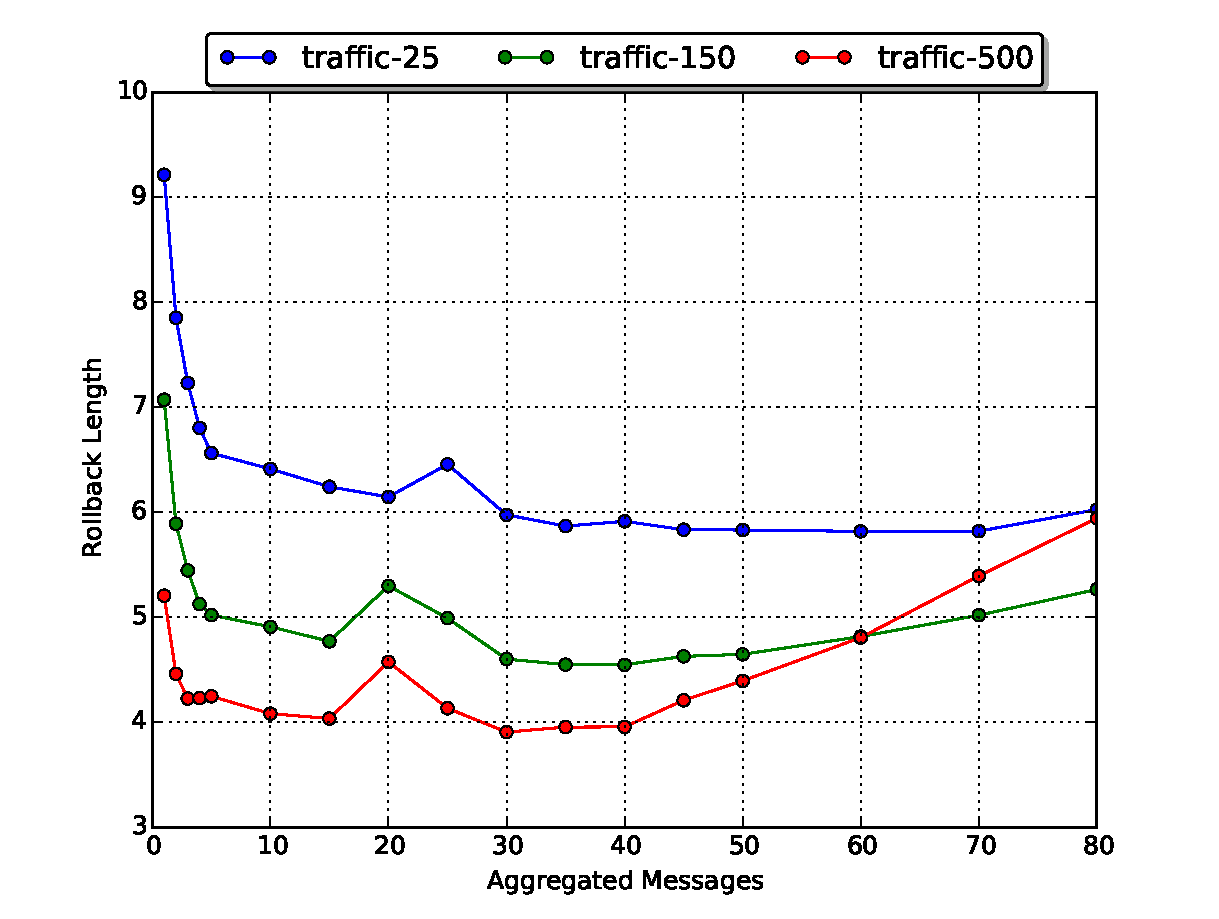
\includegraphics[width=\textwidth]{../figs/partitioning_communication/aggregate_traffic_rblength.pdf}
        \begin{itemize}
            \item Can lower rollback length?
        \end{itemize}
    \end{column}

    \end{columns}

    \bigskip

    $AverageRollbackLength = RolledBackEvents/Rollbacks$

\end{frame}

\begin{frame}{Memory Allocation - Traffic Model}
    \begin{block}{Intel\textsuperscript{\textregistered} Xeon\textsuperscript{\textregistered} X5675}
        Hyperthreading - 6 Cores, 12 Threads
        \begin{columns}
        \begin{column}{0.5\textwidth}
            \smallskip
            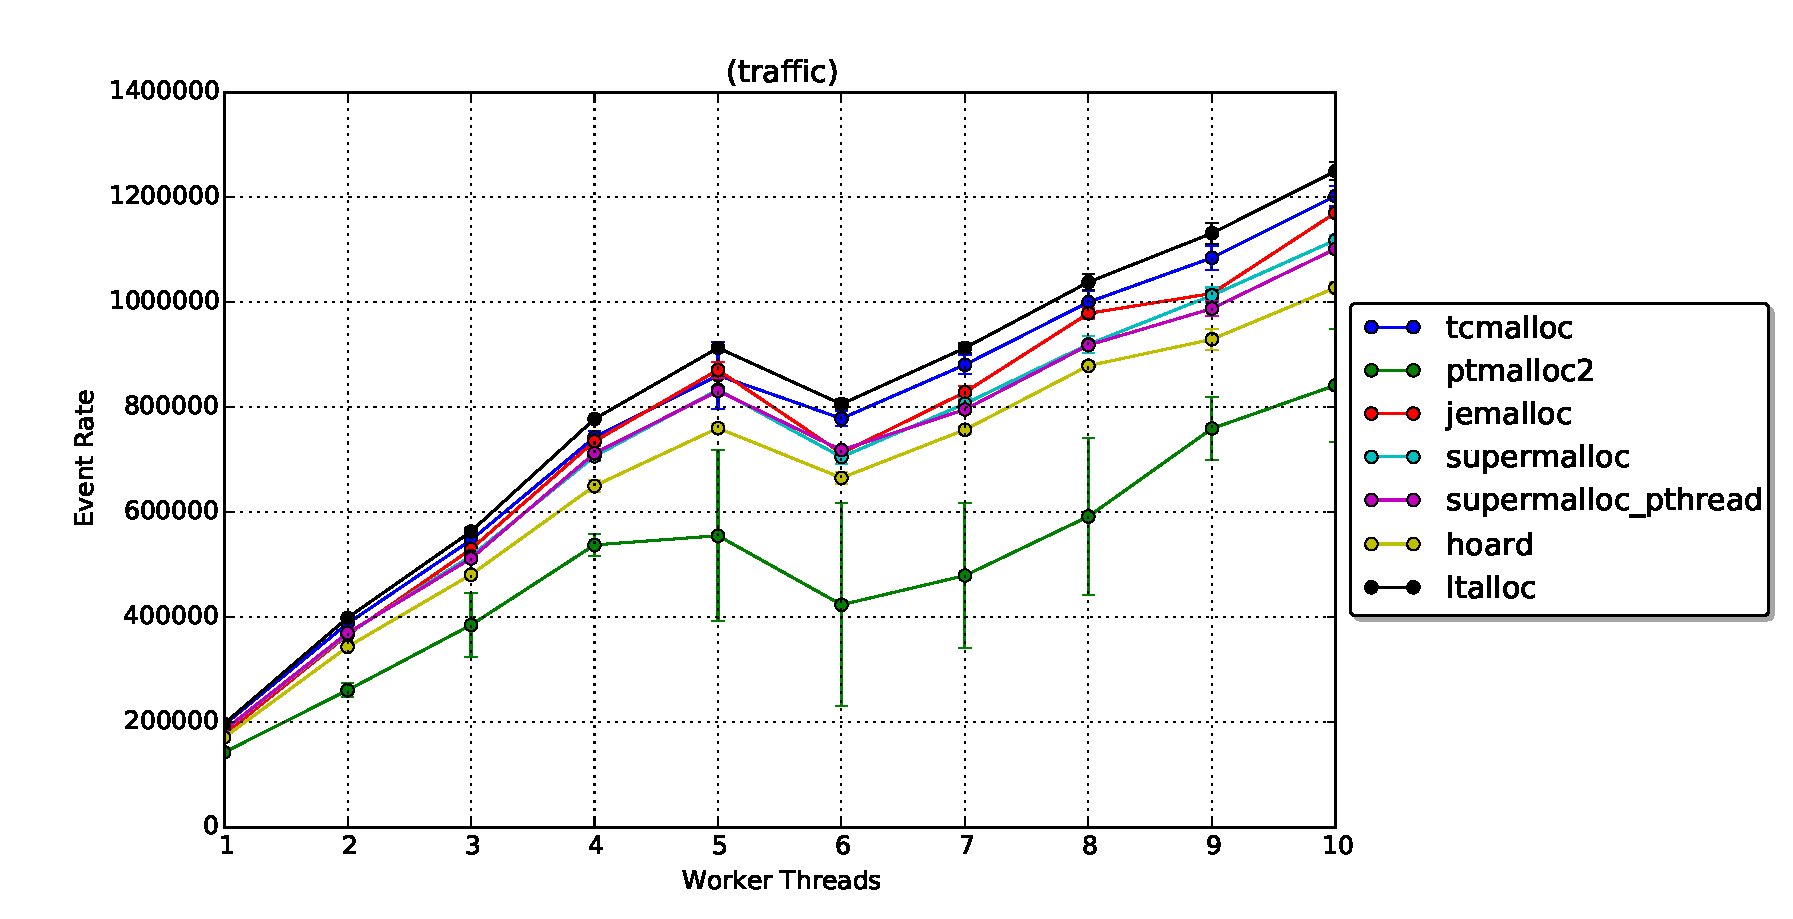
\includegraphics[width=\textwidth]{../figs/memory_allocation/traffic_eventrate.pdf} \\
            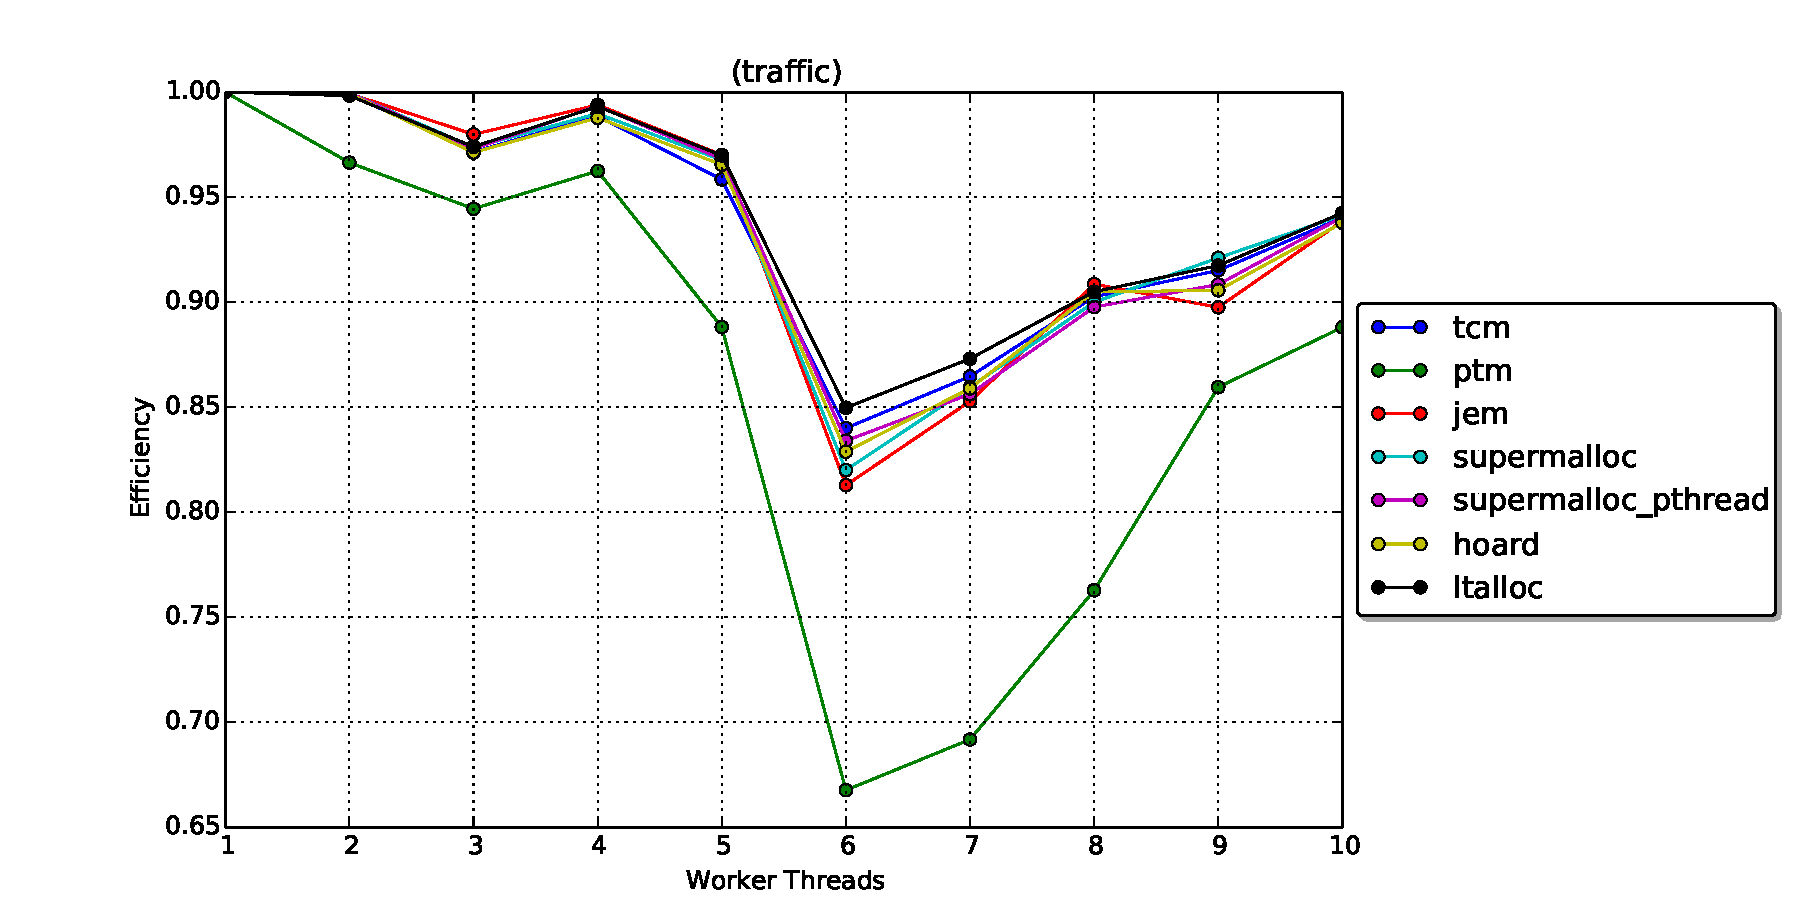
\includegraphics[width=\textwidth]{../figs/memory_allocation/traffic_efficiency.pdf} \\
        \end{column}
        \begin{column}{0.5\textwidth}
            \begin{itemize}
                \item Imbalance at 6 worker threads
                \item ptmalloc2 default in GLIBC - broken?
            \end{itemize}
        \end{column}
        \end{columns}
    \end{block}
\end{frame}

\begin{frame}{Scaling Simulation Models - Advantages}
    \begin{minipage}{0.5\textwidth}
        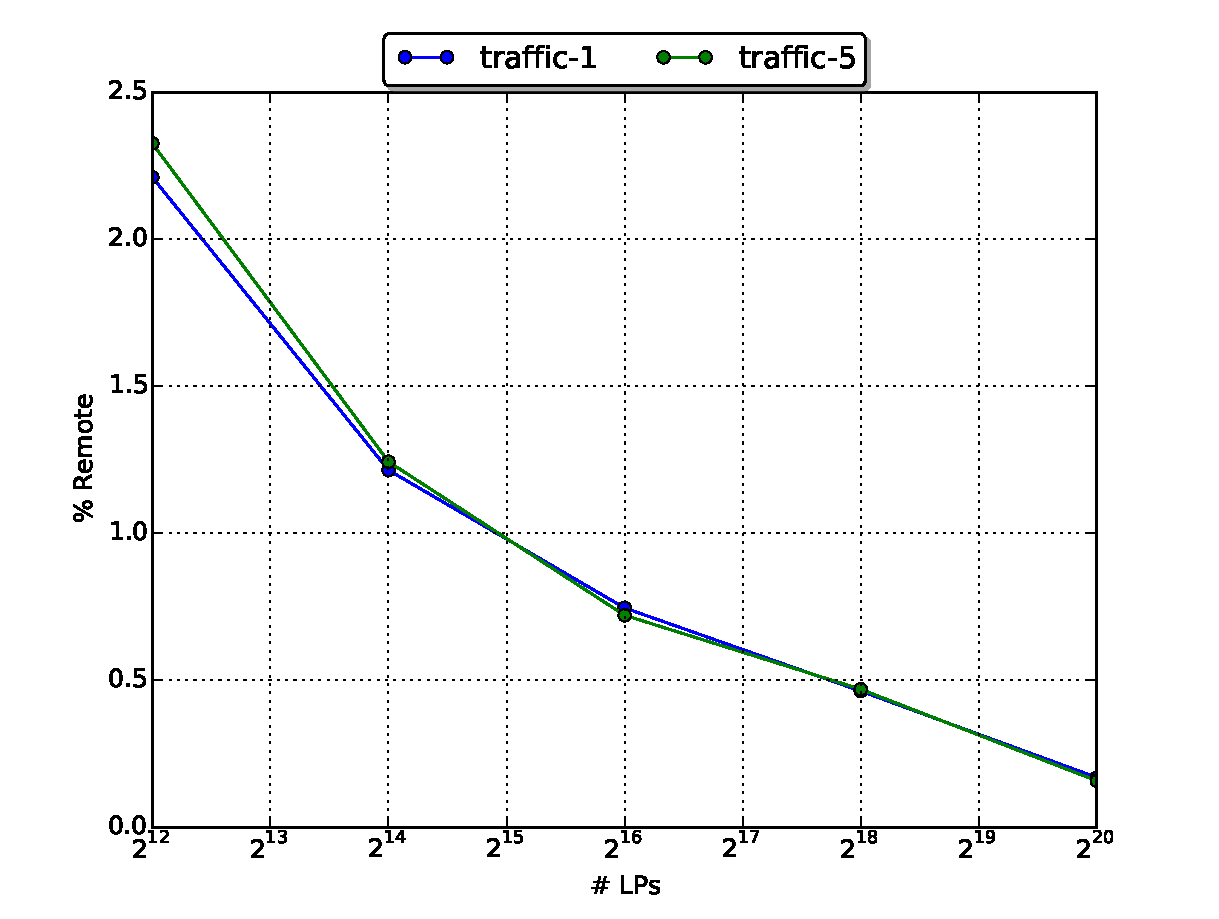
\includegraphics[width=\textwidth]{../figs/scale/scale_premote_traffic.pdf}
    \end{minipage}%
    \begin{minipage}{0.5\textwidth}
        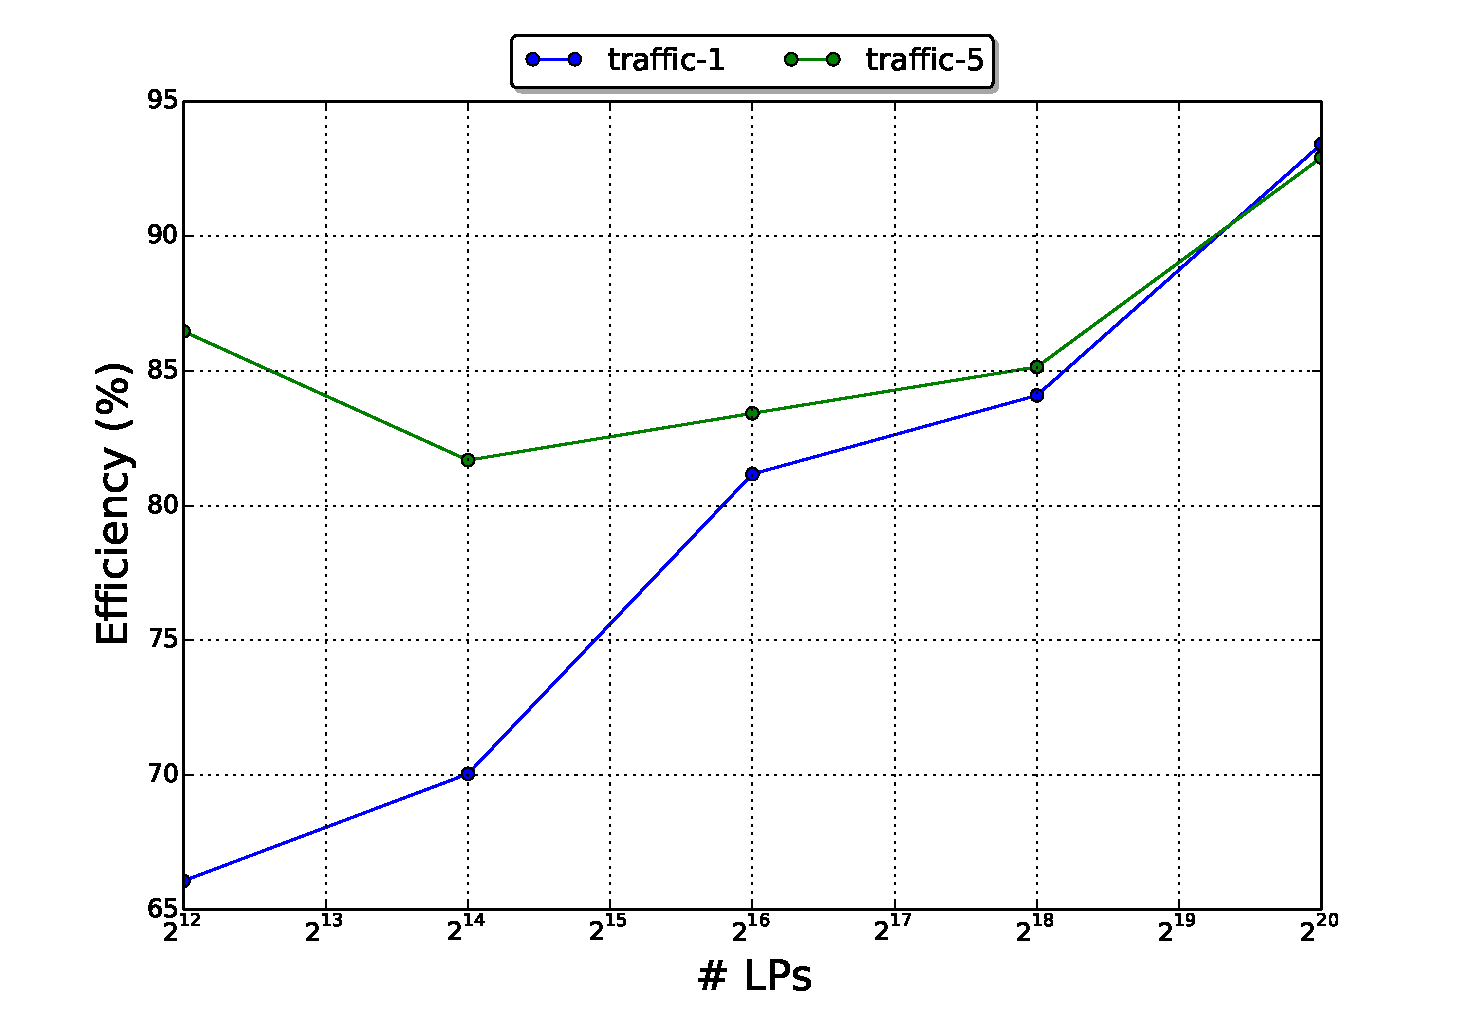
\includegraphics[width=\textwidth]{../figs/scale/scale_efficiency_traffic.pdf}
    \end{minipage}
    \begin{itemize}
        \item Coarser Granularity
        \item Higher Efficiency
    \end{itemize}
\end{frame}

\begin{frame}{Scaling Simulation Models - Disadvantages}
    \begin{minipage}{0.5\textwidth}
        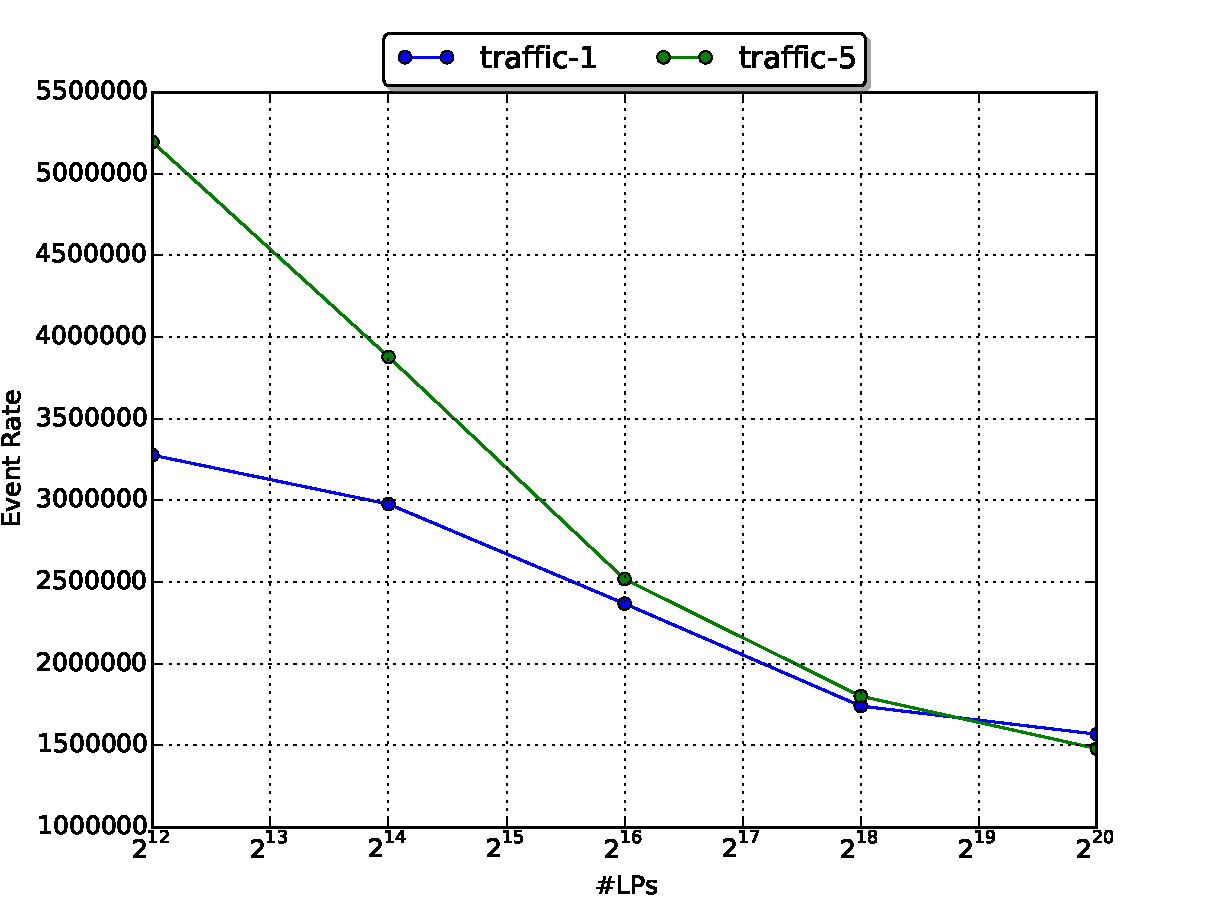
\includegraphics[width=\textwidth]{../figs/scale/scale_event_rate_traffic.pdf}
    \end{minipage}%
    \begin{minipage}{0.5\textwidth}
        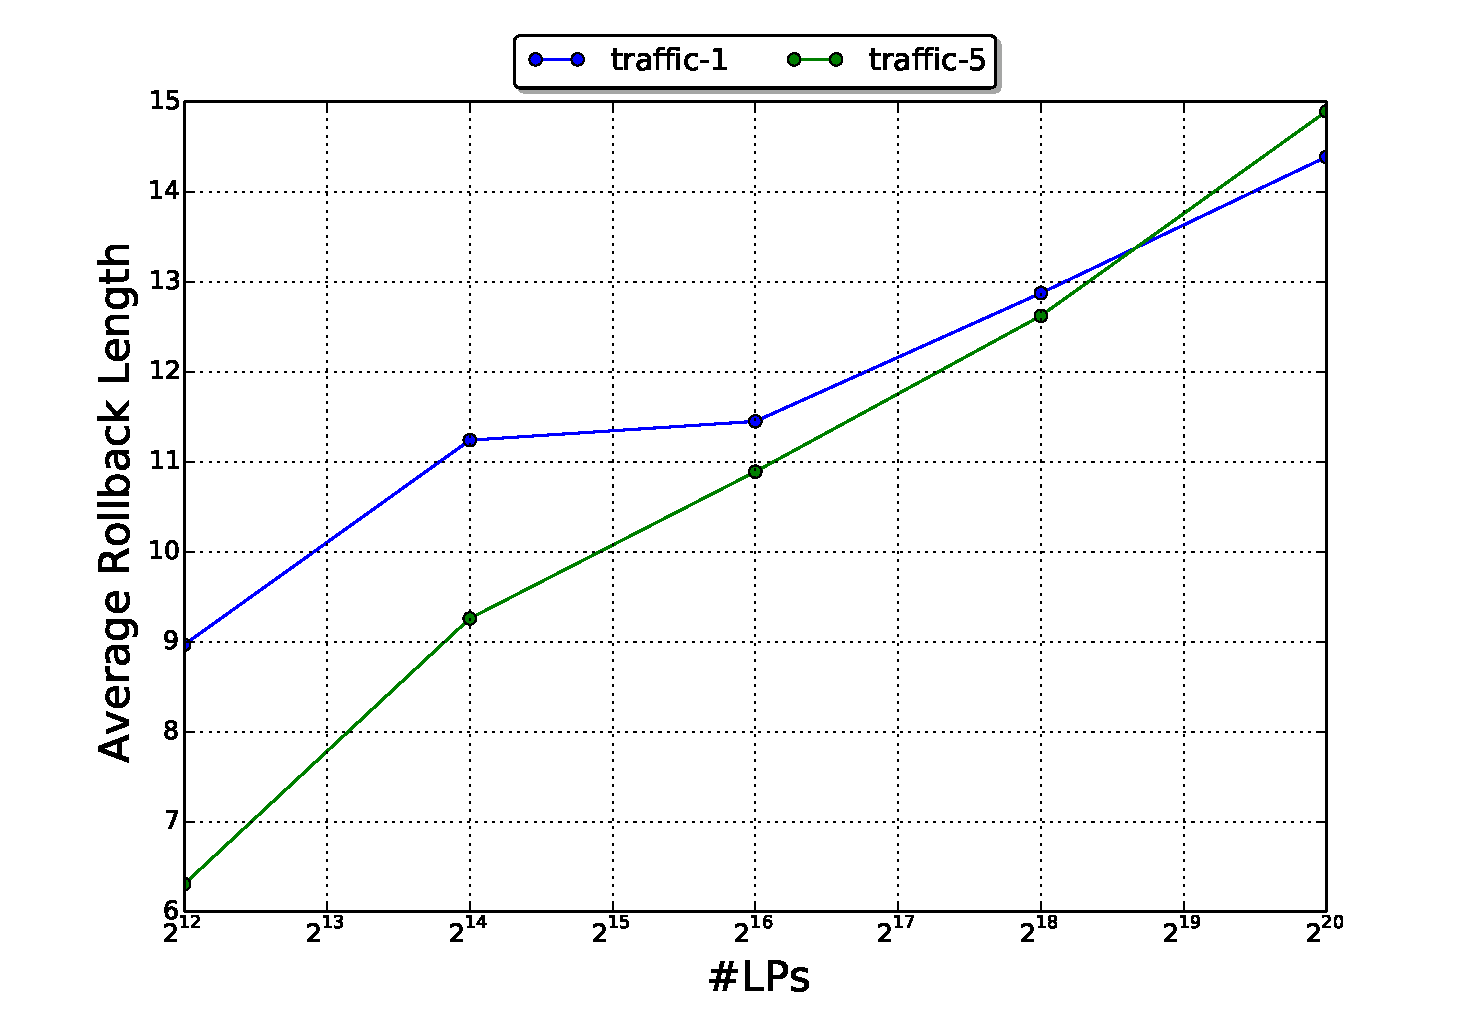
\includegraphics[width=\textwidth]{../figs/scale/scale_arl_traffic.pdf}
    \end{minipage}
    \begin{itemize}
        \item More LPs to fossil collect
        \item Longer Rollbacks
    \end{itemize}
\end{frame}

\begin{frame}{Concusionsi \& Future Research}
    \begin{itemize}
        \item Conclusions
            \begin{itemize}
                \item Synchronization should always be avoided
                    \begin{itemize}
                        \item Handle interprocess communication on a single thread
                        \item 1 LTSF queue per worker thread
                        \item 
                    \end{itemize}
                \item System can handle more rollbacks 
                \item Message aggregation works                    
                \item Memory allocation problem
            \end{itemize}
        \item Future Research
            \begin{itemize}
                \item Optimistic Fossil Collection
                \item Scaling up
            \end{itemize}
    \end{itemize}
\end{frame}

\end{document}

